\documentclass[preprint,superscriptaddress,amsmath,amssymb,aps,prl]{revtex4-1}

\usepackage{graphicx}
\usepackage{xcolor}

\newcommand{\add}[1]{\textcolor{blue}{#1}}
\newcommand{\remove}[1]{\textcolor{red}{(#1)}}

\begin{document}

 
\title{Ultrafast state detection of $^{171}Yb^+$}

\author{Ballers}
\affiliation{University of California Los Angeles}



\date{\today}

\begin{abstract}
  We do cool stuff with mode locked lasers. 
\end{abstract}

\maketitle

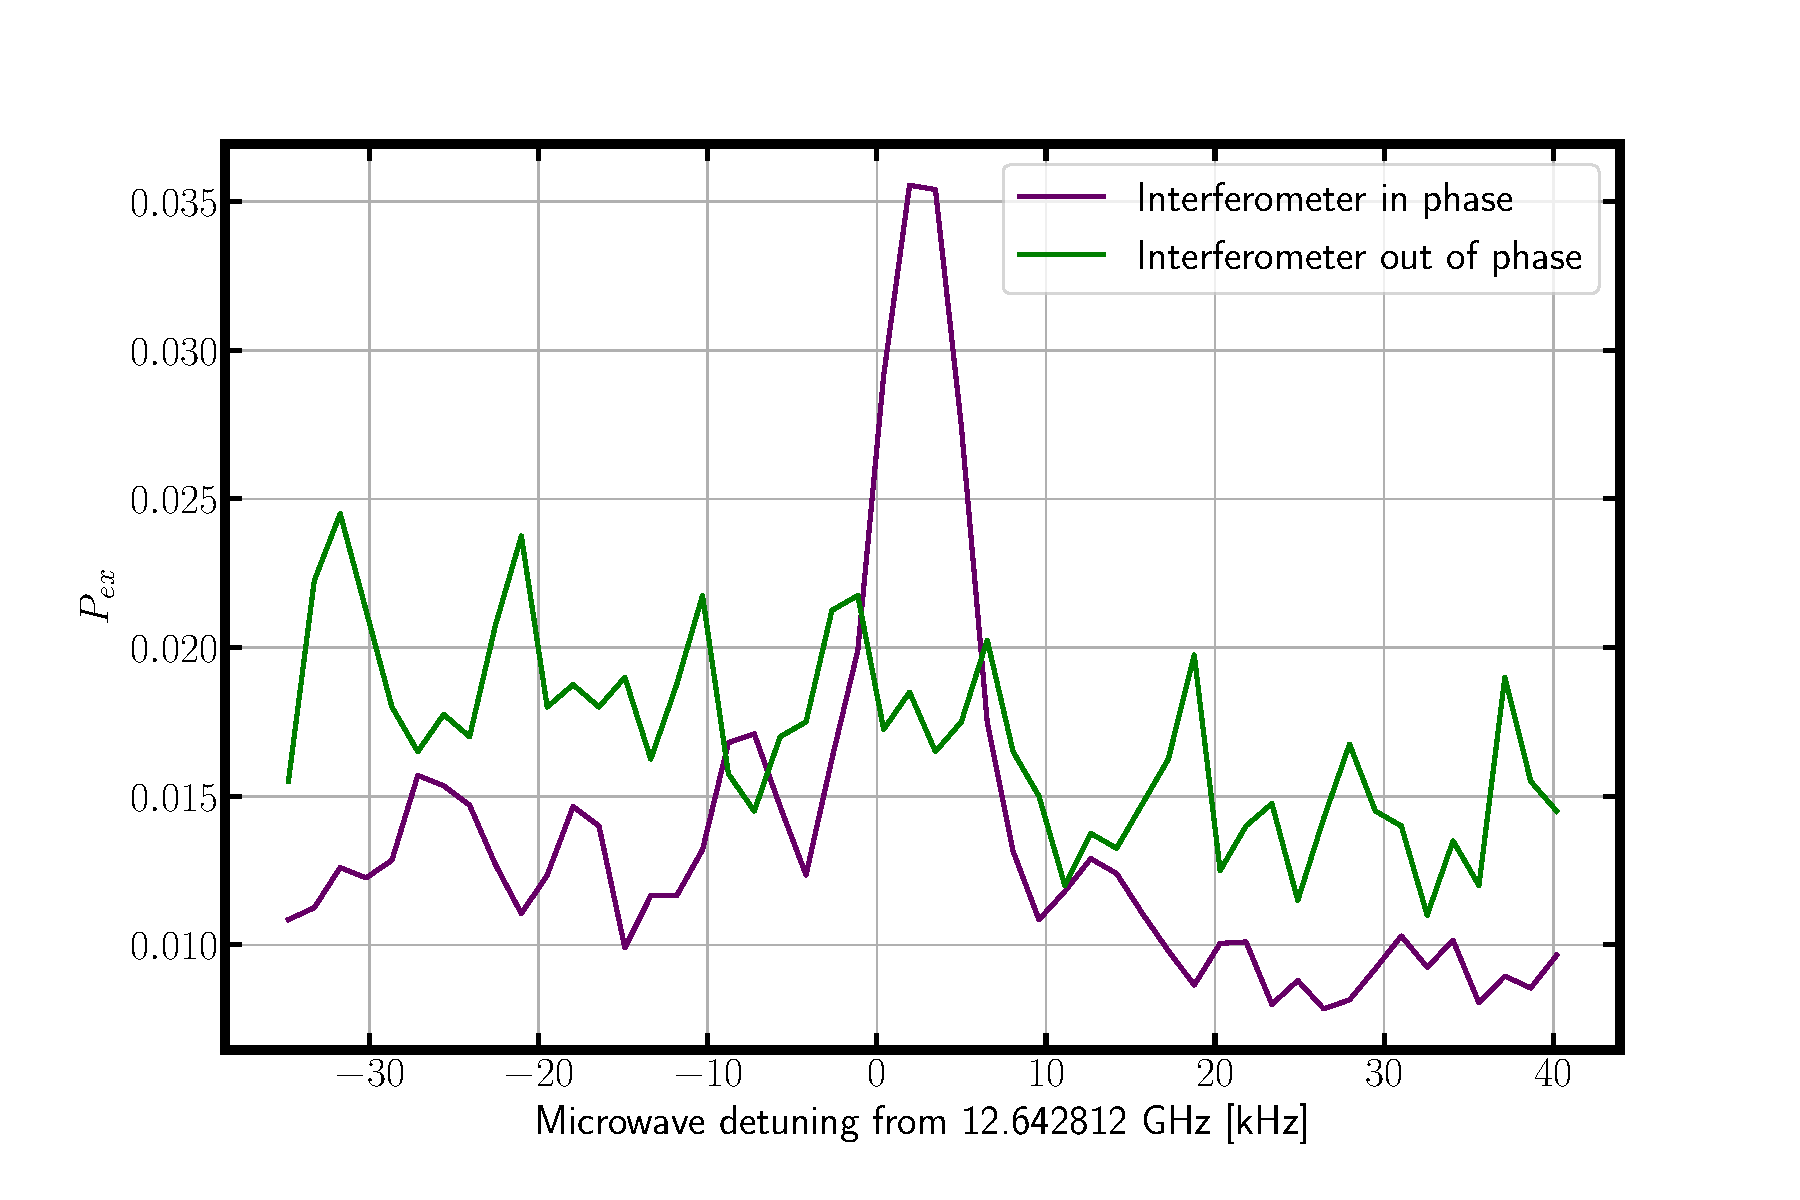
\includegraphics[scale = 0.5]{single_ion_uW_linescan_ML.pdf}

\begin{acknowledgments}
  We would like to acknowledge all of the previous ballers who laid the groundwork for our ballin' work. 
\end{acknowledgments}

\bibliography{UltrafastStateDetection}
\end{document}
